\section{The goal state, and how to read it}\label{sec:04-tactics:01-goal-state:1}

Inside \texttt{by}, Lean displays a \textbf{goal}: hypotheses above a horizontal line (named, typed facts available for use), and the statement to prove below it. Each tactic changes the goal. Sometimes it closes the goal, sometimes it splits it into several smaller goals, and sometimes it merely rewrites it into an equivalent but easier-to-handle shape. Proving something in Lean is mostly the skill of examining the current goal and asking: \emph{what tactic changes this into something closer to solved?}

\begin{lstlisting}
theorem two_plus_two : 2 + 2 = 4 := by
  rfl
\end{lstlisting}

Placing the cursor after \texttt{by} in an editor with the Lean extension shows the goal:

\begin{lstlisting}
⊢ 2 + 2 = 4
\end{lstlisting}

No hypotheses, one goal. After \href{https://lean-lang.org/doc/reference/latest/Tactic-Proofs/Tactic-Reference/}{\texttt{rfl}} closes it, the goal panel shows ``No goals''. The proof is complete.

\begin{mathreading}

A goal is what logicians call a \emph{sequent}: a list of hypotheses together with a statement to prove from them. A tactic is a \emph{backward inference rule}. It replaces the current goal with zero or more simpler goals whose proofs would be enough to prove it. This is exactly the mathematician's habit of saying ``it suffices to show\ldots{}''. Closing every goal means a complete chain of such steps has been built down to something already known. Here, that chain is just one step: \texttt{2 + 2 = 4} by plain computation.

\end{mathreading}

\begin{quote}
Read more: if ``sequent'' or ``backward inference rule'' are new, \hyperref[sec:03-propositions-and-proofs:02-logic-recap:1]{Chapter 3 §2} recaps natural deduction --- the standard proof system these words describe, turnstile notation and all --- from scratch, with no Lean involved.
\end{quote}

\textbf{The goal state should be checked after every tactic}, not just at the end. This is the chief difference between someone who can read a finished Lean proof and someone who can write one. Writing one requires constantly asking ``what does the goal look like \emph{now}, and what would make progress on \emph{this exact shape}?''

\section{A worked strategy session, before any new tactics}\label{sec:04-tactics:01-goal-state:2}

Suppose the task is to prove \texttt{(a b : Nat) → a + b = b + a}, with the proof not yet known. What follows is the actual thought process, not the polished result.

\begin{enumerate}
\def\labelenumi{\arabic{enumi}.}
\item
  \textbf{Try the cheapest thing first.} \texttt{rfl} asks ``do both sides already compute to the same normal form?'' For \texttt{a + b = b + a} with \texttt{a}, \texttt{b} as variables (not concrete numbers), the answer is no. \texttt{Nat.add} recurses on its \emph{second} argument, so \texttt{a + b} and \texttt{b + a} do not reduce to a common form without knowing more about \texttt{a} and \texttt{b}. \texttt{rfl} fails with an error such as ``motive is not type correct'' or ``type mismatch.'' That failure is \emph{information}: it indicates the equality is not definitional, hence an actual argument is required, not just unfolding.
\item
  \textbf{Look for structure to induct or case-split on.} Both sides mention \texttt{a} and \texttt{b} as \texttt{Nat}s, and \texttt{Nat} is inductively defined (Chapter 1), so induction is the natural move. The question becomes \emph{which} variable to induct on. Trying \href{https://lean-lang.org/doc/reference/latest/Tactic-Proofs/Tactic-Reference/}{\texttt{induction b}} is suggested by the recursion on \texttt{+}'s second argument, since \texttt{b} is the one that unfolds cleanly.
\item
  \textbf{Read the two resulting goals.} After \texttt{induction b with | zero => \_ | succ k ih => \_} there is a \texttt{zero} goal, \texttt{a + 0 = 0 + a}, and a \texttt{succ} goal, \texttt{a + (k+1) = (k+1) + a} with hypothesis \texttt{ih : a + k = k + a} available. Neither is \texttt{rfl} on the nose (again, this is checked by trying it; if it fails, that indicates a helper fact is missing), so each needs its own small rewrite, using lemmas about how \texttt{+} unfolds on \texttt{zero}/\texttt{succ}.

  This is exactly what the editor shows, live, as the proof is worked: the cursor sits right before \texttt{rw [Nat.add\_succ]} in the \texttt{succ} case, and the \textbf{Lean Infoview} panel on the right lists the hypotheses (\texttt{a k : Nat}, \texttt{ih : a + k = k + a}) above the line and the current goal (\texttt{a + (k + 1) = k + 1 + a}) below it --- precisely the ``hypotheses above a horizontal line, goal below it'' picture described above, not merely a text mock-up of it:

  \begin{figure}
  \centering
  \pandocbounded{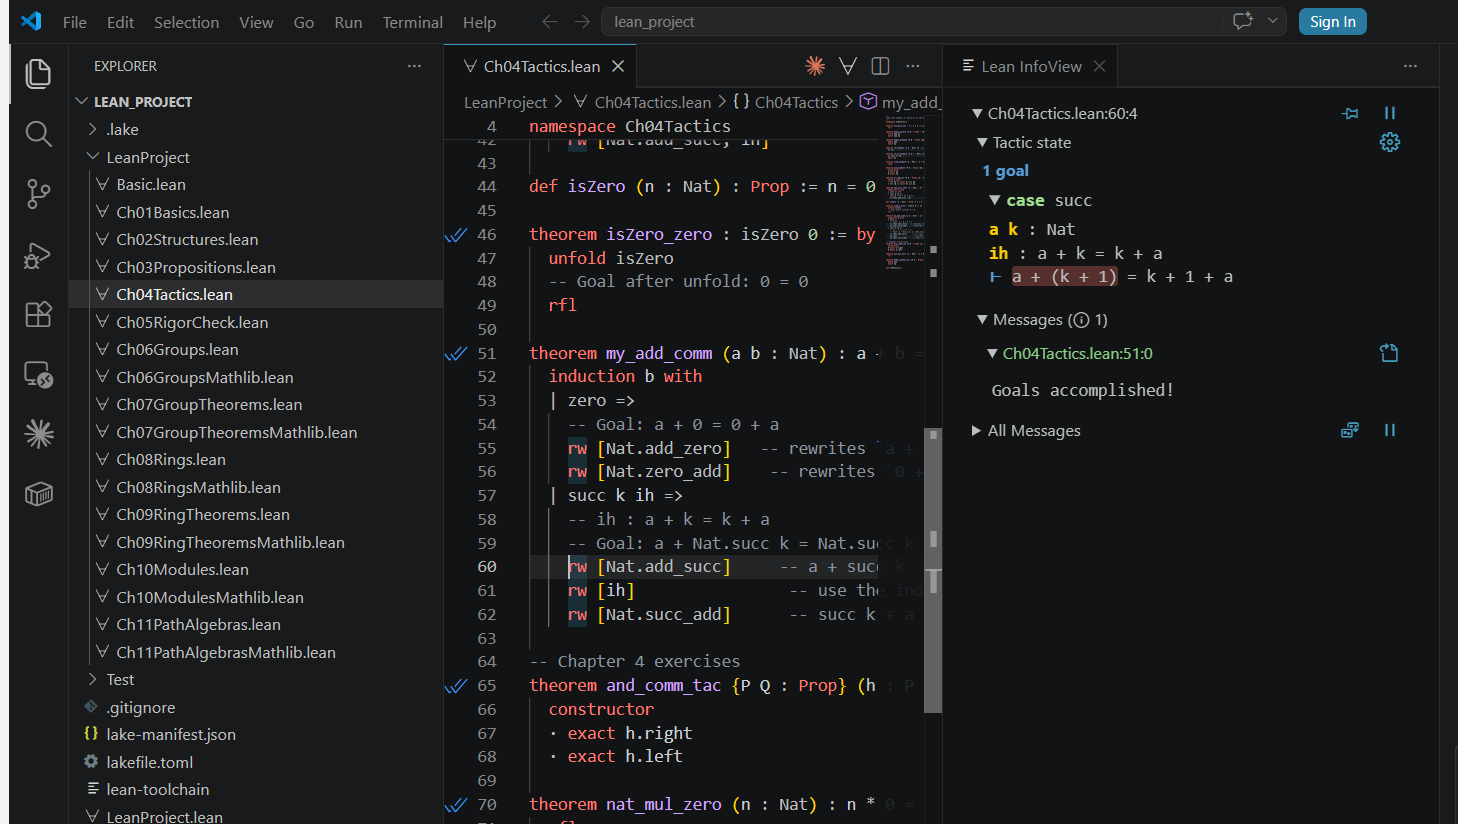
\includegraphics[keepaspectratio,alt={The Lean Infoview panel in VS Code, showing the tactic state (hypotheses a k : Nat, ih : a + k = k + a, goal a + (k + 1) = k + 1 + a) for the succ case of my\_add\_comm's induction.}]{../04-tactics/images/goal-state-infoview.png}}
  \caption{The Lean Infoview panel in VS Code, showing the tactic state (hypotheses \protect\texttt{a k : Nat}, \protect\texttt{ih : a + k = k + a}, goal \protect\texttt{a + (k + 1) = k + 1 + a}) for the \protect\texttt{succ} case of \protect\texttt{my\_add\_comm}'s induction.}
  \end{figure}
\item
  \textbf{Find the missing lemmas.} \texttt{Nat.add\_succ} and \texttt{Nat.zero\_add} need not be memorized. In an editor, typing \texttt{rw [Nat.add\_} and using autocomplete lists everything starting that way. Alternatively, \href{https://lean-lang.org/doc/reference/latest/Tactic-Proofs/Tactic-Reference/}{\texttt{exact?}} (Chapter 12), searches the whole environment for something that closes the current goal outright, and will often name exactly the lemma required even when its name cannot be guessed.
\end{enumerate}

This four-step loop --- \emph{try the cheap tactic, determine why it failed, find structure to split on, locate the specific lemma matching the resulting shape} --- is the real content of ``knowing Lean.'' The worked-out proof later in this chapter, and every proof in Chapters 5--9, is the \emph{output} of this loop. What matters is the loop, not merely the output.
